\section{现有时间隐通道构造方案}
\label{chap:backinfo:ctc}

%概述,在以太网中进行时间隐通道的研究已经有成果
基于以太网的时间隐通道,是隐通道研究中一个非常重要的课题。随着计算机网络的发展,基于单主机的时间隐通道,已经难以满足隐蔽传输的需求,借助计算机网络高带宽、大流量的优势,时间隐通道在传输性能、隐蔽性方面有了进一步的提升。
%在移动互联网下的方案,也已经存在
当前移动互联网已经成为主流,面向移动终端的流媒体应用及实时通信应用兴起,这些场景的出现,为时间隐通道的构建方法提供了新的思路。
%这些方案中有一些通用的方法及保证鲁棒性的策略
时间隐通道需要面对的一个共同难题,是如何在噪声干扰下保证传输鲁棒性,提高时间隐通道可用性。作为寄生信道,时间隐通道在信噪比水平方面,与宿主信道有很大差距,在方法设计的原理和优化过程中,需要针对性改进。

\subsection{基于以太网的时间隐通道构造方案}
\label{chap:backinfo:ctc:ethernet}
%经典时间隐通道
%IPD-CTC
基于以太网的时间隐通道,通常通过调整时间或数据包序号,突破系统中的安全级别限制,实现隐蔽消息的传输。此外,如果时间隐通道利用了其他时间特征,检测上极为困难。

\insertFigure{
	\begin{figure}
		\centering
        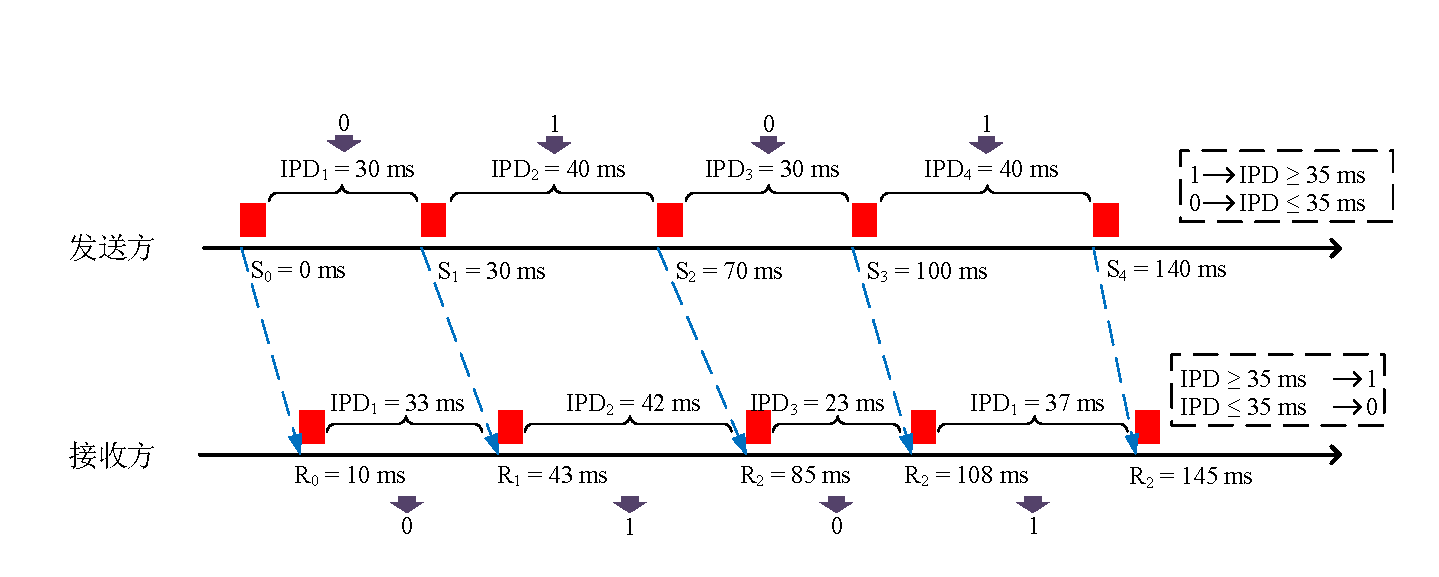
\includegraphics[width=0.99\textwidth]{chapters/chapter2/figures/ipd-ctc.pdf}
        \caption{基于IPD的时间隐通道示意图}\label{fig:2:ipd-ctc}
	\end{figure}
}

数据包的传输过程,存在传输时间间隔的特性,利用该特性构造的时间隐通道,成为基于IPD的时间隐通道。\nupcite{4317620,8600755,WALLS20111217}如图\nref{fig:2:ipd-ctc},双方选择的宿主信道平均IPD为35ms,待发送的二进制数据序列为$\{0, 1, 0, 1, \cdots\}$。对于发送方来说,需要传输1时,需要将当前的IPD设定为35以上;需要传输0时,将当前的IPD设定为35以内。图中根据数据包缓冲区的内容,及待发送的数据信息,对数据包的发送时刻进行调整,完成调制过程。当经过网络传输后,受噪声及传输调度的影响,数据包接收的时间间隔出现畸变。接收方使用相同的规则进行解调,得到隐蔽消息,如果噪声太强,则接收消息会出现误码。

%on-off CTC
\insertFigure{
	\begin{figure}
		\centering
        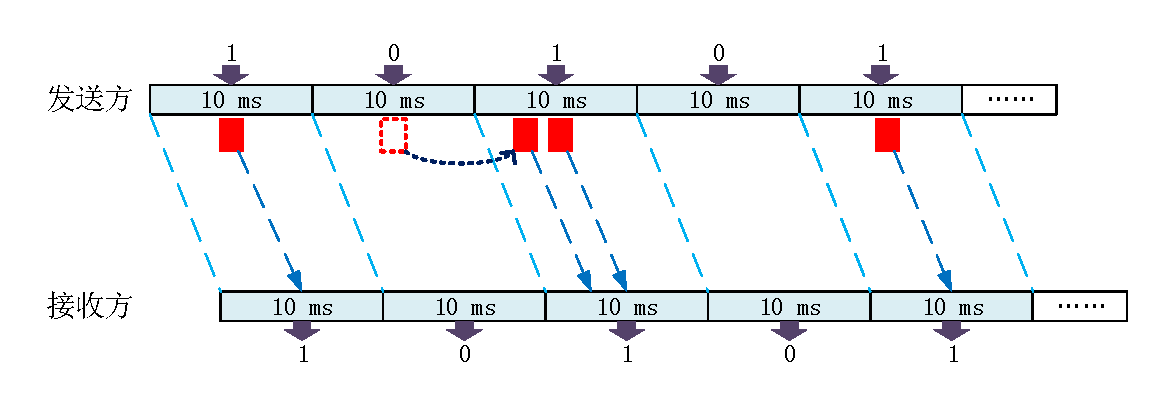
\includegraphics[width=0.9\textwidth]{chapters/chapter2/figures/onoff-ctc.pdf}
        \caption{基于On/Off模式的时间隐通道示意图}\label{fig:2:onoff-ctc}
	\end{figure}
}
另一种典型的时间隐通道为On/Off模式的时间隐通道,类似于开关的开关状态,任意时刻只有两种状态中的一种,通过控制数据包的是否传输,实现时间隐通道的构造。\nupcite{Cabuk:2004:ICT:1030083.1030108,5062145,6406084}如图\nref{fig:2:onoff-ctc},发送方与接收方按照10 ms的时间窗口,控制在窗口内是否发送数据包,发送的代表传输1,不发送则代表传输0。在这类时间隐通道中,隐蔽消息的编码适用不归零编码,利用时钟作为信号同步。

%Model-based CTC
\insertFigure{
	\begin{figure}
		\centering
        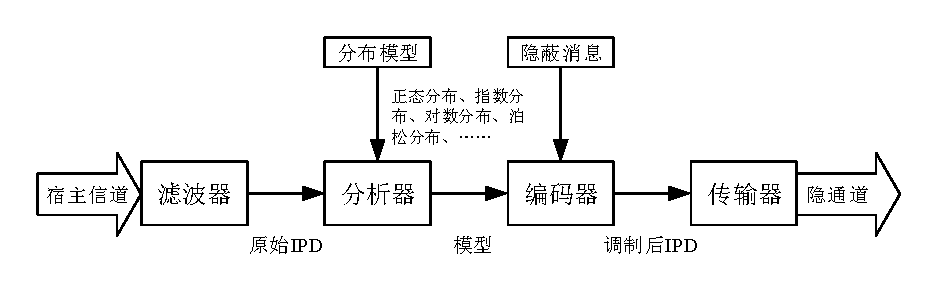
\includegraphics[width=0.85\textwidth]{chapters/chapter2/figures/mb-ctc.pdf}
        \caption{基于模型的时间隐通道示意图}\label{fig:2:mb-ctc}
	\end{figure}
}
基于模型的时间用通道,通过建模宿主信道的传输特征,以模拟的方式拟合已知分布,从而避免被监听者察觉。构建基于模型的时间隐通道,首先需要对拟合目标进行建模,创建拟合目标。\nupcite{5062145,ahsan2002practical}在隐通道的调制阶段,通常包含滤波器、分析器、编码器及传输器几个部分,实现对宿主信道的调整,完成隐通道的构建。如图\nref{fig:2:mb-ctc},滤波器分析宿主信道中的IPD特征,并将分析结果传送给分析器。分析器根据已知的模型特征,分析当前适配的模型类型。编码器利用该模型,借助分布函数及累积分布函数,将隐蔽消息编码进IPD中。传输器根据目标IPD,调整宿主信道的发送间隔,完成隐通道的构建。

\subsection{基于移动互联网的时间隐通道构造方案}
\label{chap:backinfo:ctc:mobile}
%介绍Skype、VoIP等构造方案
在移动互联网环境下,时间隐通道的构造方法,与以太网环境下的时间隐通道有相似点。面向移动互联网的应用环境,数据包传输特征发生了变化,基于以太网的时间隐通道构建方法,无法满足隐蔽性方面的需求。

\insertFigure{
	\begin{figure}
		\centering
        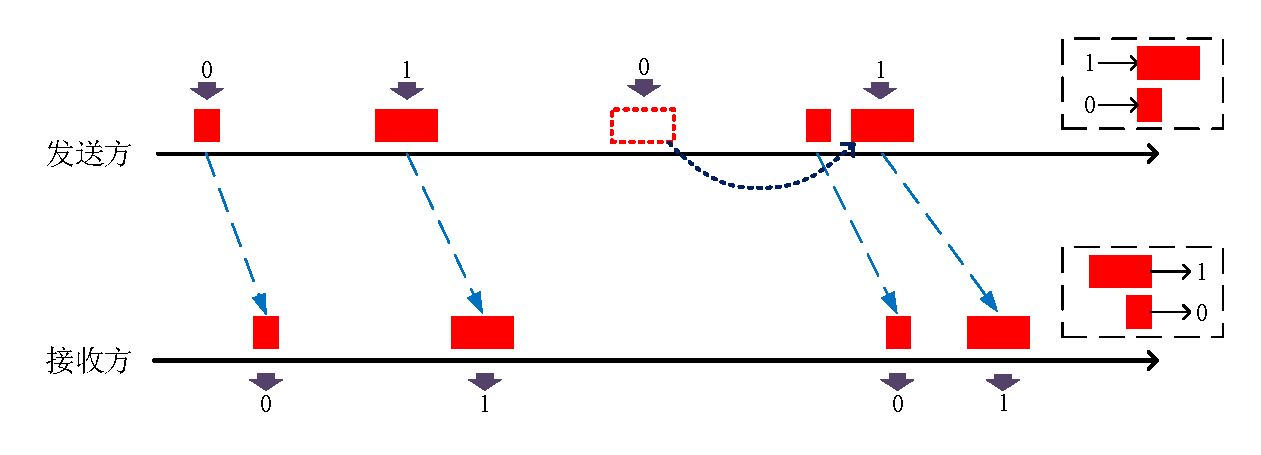
\includegraphics[width=0.95\textwidth]{chapters/chapter2/figures/pl-ctc.pdf}
        \caption{基于数据包长度的时间隐通道示意图}\label{fig:2:pl-ctc}
	\end{figure}
}

%Packet-Length CTC。 Liang
对于VoIP等实时交互应用,数据包长度并不是完全随机的,根据实际数据传输的需求不断变化。通过统计数据包长度的分类情况,划分出独立的编码符号,在发送过程中,根据缓冲区中数据包的内容,及当前数据需求,调整数据包传输顺序,完成隐蔽消息嵌入。\nupcite{LIANG2018144,8277839}如图\nref{fig:2:pl-ctc},通过调整数据包的发送顺序,根据隐蔽消息的发送需求构造数据包序列。

%Packet-content CTC, 长度的奇偶
对于移动互联网中的数据包,尤其是基于RTP的数据包来说,在一次通信过程中,数据包的内容应该都是唯一的,出现HASH冲突的概率非常低。除了借助数据包传输特征,数据包自身的特征也构成了连续不断的特征流。借助信息摘要算法,计算数据包负载的特征,并利用其中特定位置的结果,作为数据包特征的标记。通过调整不同标记数据包的位置,完成调制过程的消息嵌入,实现隐通道构建。\nupcite{LIANG2018162,6670985}

%VoLTE RTP、RTCP CTC
对于VoLTE来说,由于采用了基于RTP的传输方案,需要通过RTCP数据包完成传输反馈。这两种同时存在的数据包,形成了构建时间隐通道的传输特征。RTCP数据包的数量较少,发送过程比较离散,通过调整RTCP数据包之间的RTP数据包的数量,将隐蔽消息嵌入到RTP数据包数量中,构建时间隐通道的方法是有效的。\nupcite{ZHANG201866}

\insertFigure{
	\begin{figure}
		\centering
        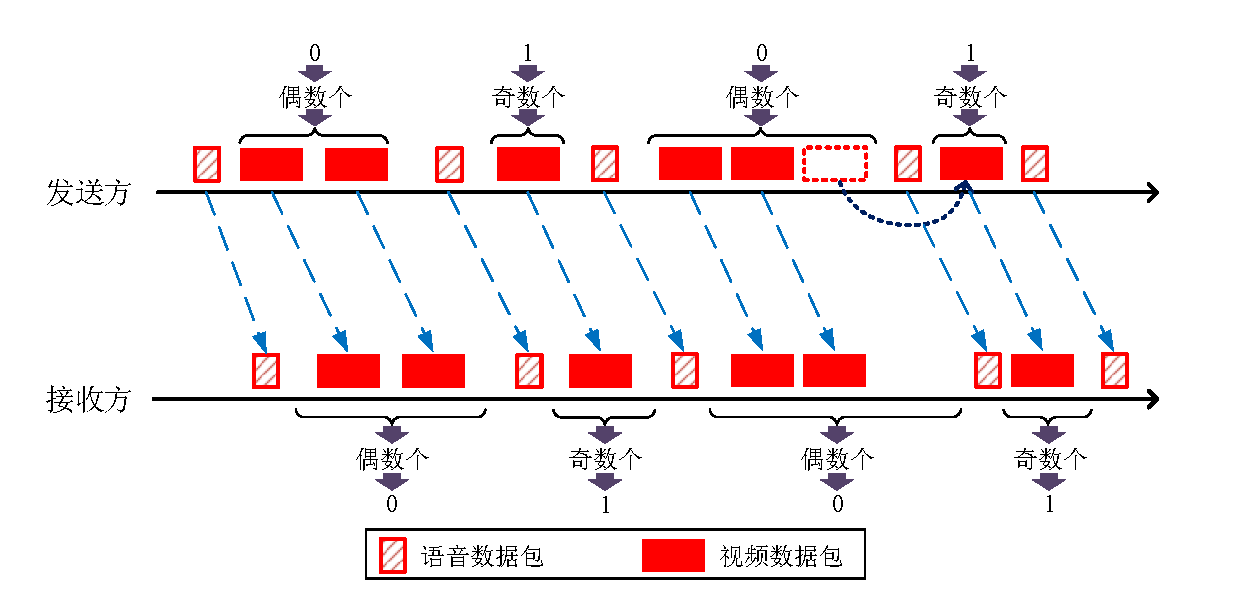
\includegraphics[width=0.9\textwidth]{chapters/chapter2/figures/av-ctc.pdf}
        \caption{基于数据包计数的时间隐通道示意图}\label{fig:2:av-ctc}
	\end{figure}
}

%VoLTE Video、Audio CTC
类似于RTP及RTCP的方案\nupcite{ZHANG201866},参考图\nref{fig:2:ap-bp},语音数据包和视频数据包最终都由BP进行处理,在BP一侧,语音数据包具有明显的时间规律,作为参照时钟信号。语音数据包之间间隔的视频数据包数量,随时间段产生变化,AMR-WB语音编码时,语音数据包每20 ms发送一次。另一方面,30 fps时视频的采样周期大约为33 ms,视频数据包与语音数据包发送周期不同步,调整语音数据包之间视频数据包数量的方法,符合传输隐蔽性的要求。该模式的示意图如图\nref{fig:2:av-ctc},需要调整的数据包数量少,具有良好的抗检测能力。

\subsection{时间隐通道的鲁棒性策略}
\label{chap:backinfo:ctc:robustness}
正如\nref{chap:backinfo:ctc}所述,时间隐通道在鲁棒性方面需要格外重视。常用的鲁棒性方法,包括鲁棒性编码、附加校验及纠错信息等。不同的方法各有优势,在应用中通常与噪声类型结合,根据去噪需求采用对应的方法。

%介绍各个方案中,为保证鲁棒性,采用的检错、纠错编码,重传策略等
%Gray码
\insertTable{
	\begin{table}[]
        \centering
        \caption{格雷码编码表}
        \label{tab:2:gray-code}
        \begin{tabular*}{0.6\textwidth}{@{\extracolsep{\fill}}cccc}
        \toprule
        数据 & 1 bit格雷码 & 2 bit格雷码 & 3 bit格雷码\\ 
        \midrule
        0 & 0 & 00 & 000 \\ 
        1 & 1 & 01 & 001 \\ 
        2 &   & 11 & 011 \\ 
        3 &   & 10 & 010 \\ 
        4 &   &    & 110 \\ 
        5 &   &    & 111 \\ 
        6 &   &    & 101 \\ 
        7 &   &    & 100 \\ 
        \bottomrule
        \end{tabular*}
    \end{table}
}

\insertFigure{
	\begin{figure}
		\centering
        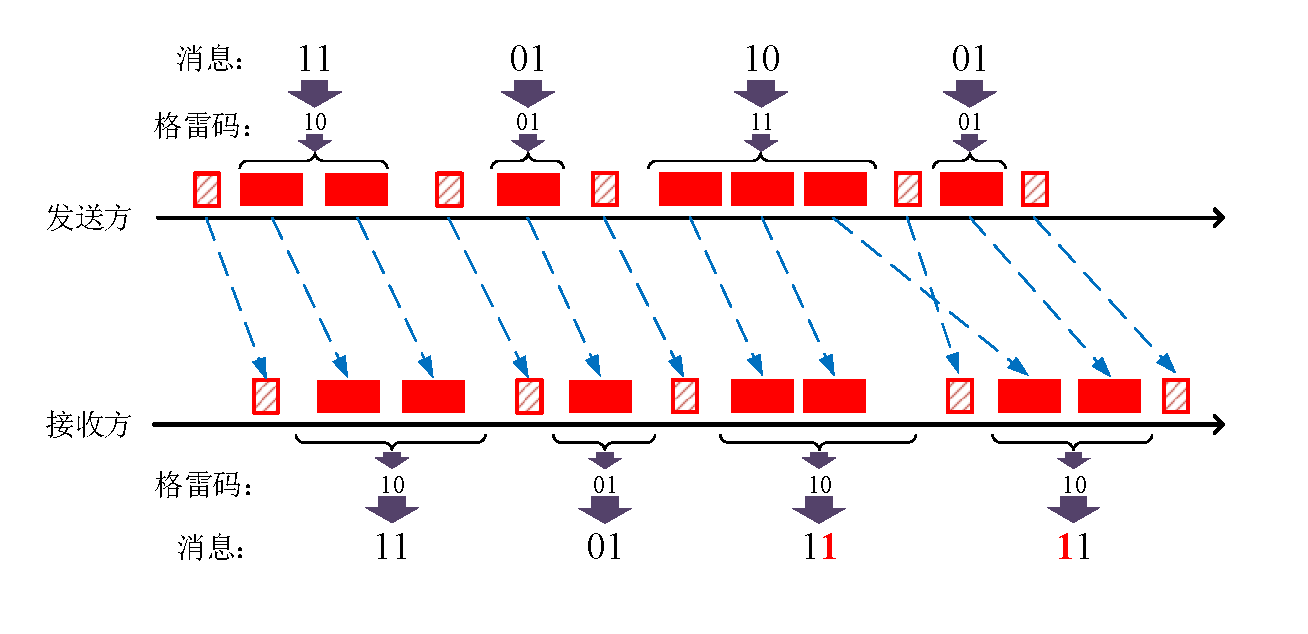
\includegraphics[width=0.9\textwidth]{chapters/chapter2/figures/gray-ctc.pdf}
        \caption{基于格雷码的时间隐通道鲁棒性示意图}\label{fig:2:gray-ctc}
	\end{figure}
}

格雷码又称循环二进制单位距离码,任意两个相邻数的代码只有一位二进制数不同,与叫偶校验码同属于可靠性编码。\nupcite{7329924}不同位数的格雷码如表\nref{tab:2:gray-code}所示,利用相邻数据码小的优势,当统计误差只有$\pm1$时,接收到的错误只会有一位,减少了误码的位数。格雷码的应用优势如图
\nref{fig:2:gray-ctc}%替换
,发送方使用间隔数据包数量的方法进行调制,接收过程中出现不可预期的乱序时,格雷码能够抑制噪声。\nupcite{8600755,8817935}

%Guard Band
受网络噪声的影响,编码符号之间的区分难度增大,符号之间设定一定长度的缓冲区,实现符号与噪声的隔离。当监测到的符号落入缓冲区间时,视为噪声丢弃,否则处理后将产生显著的误码。根据符号的类型,缓冲区设定为单个\nupcite{6567004,6296078},或设定为多个\nupcite{LIANG2018162},对应的是各符号的有效范围。

%喷泉码等
除了以上方法,一些特殊的编码算法,也应用在了时间隐通道中。基于喷泉码的时间隐通道,使用随机生成的关系矩阵,完成原始数据符号的线性编码。该方法保证了每个符号中有足够的冗余信息,结合抹除码的特征,在正确接收符号的前提下,具有较好的保密性和鲁棒性。\nupcite{6296078}除了喷泉码,低密度奇偶校验码、里所码、卷积码、Turbo码均在一定程度上提升了鲁棒性。\nupcite{10.1007/978-3-642-24178-9_22}

\subsection{讨论}
在VoLTE场景中,存在的噪声只有丢包和乱序两种,基于主动丢包的时间隐通道,隐匿在丢包噪声中,在构造的基本原理上与原有的时间隐通道存在区别。现有的时间隐通道鲁棒性策略,主要是抵御网络噪声及防守方,带来的少量干扰。对于本论文的时间隐通道构建方法来说,更重要的是将微弱的信号从噪声背景中筛选出来,并且解调过程无法确保监测符号的正确性,可靠性编码不能解决该问题,需要设计一种内部交叉校验的鲁棒性方法。